% !TeX spellcheck = sk_SK-Slovak
\documentclass[a4paper]{article}
\usepackage[slovak]{babel}
\usepackage[utf8]{inputenc}
\usepackage[T1]{fontenc}
\usepackage{a4wide}
\usepackage{amsmath}
\usepackage{amsfonts}
\usepackage{amssymb}
\usepackage{mathrsfs}
\usepackage[small,bf]{caption}
\usepackage{subcaption}
\usepackage{xcolor}
\usepackage{graphicx}
\usepackage{enumerate}
\usepackage{hyperref}



\pagestyle{empty}
\setlength{\parindent}{0pt}

\newenvironment{modenumerate}
{\enumerate\setupmodenumerate}
{\endenumerate}

\newif\ifmoditem
\newcommand{\setupmodenumerate}{%
	\global\moditemfalse
	\let\origmakelabel\makelabel
	\def\moditem##1{\global\moditemtrue\def\mesymbol{##1}\item}%
	\def\makelabel##1{%
		\origmakelabel{##1\ifmoditem\rlap{\mesymbol}\fi\enspace}%
		\global\moditemfalse}%
}

\begin{document} 
	
\pagenumbering{arabic}
\pagestyle{plain}

\begin{center}
	\sc\large
	VEDA O SIEŤACH / ALGORITMY NA SIEŤACH 2023
	DOMÁCA ÚLOHA 2
\end{center}

Autor: Marián Kravec

\section{Úloha 1}

\begin{enumerate}[(a)]
	\item 
	V prípade pozorovaného správania mravcov vyzerala výsledná sieť následovne:
	
	\centerline{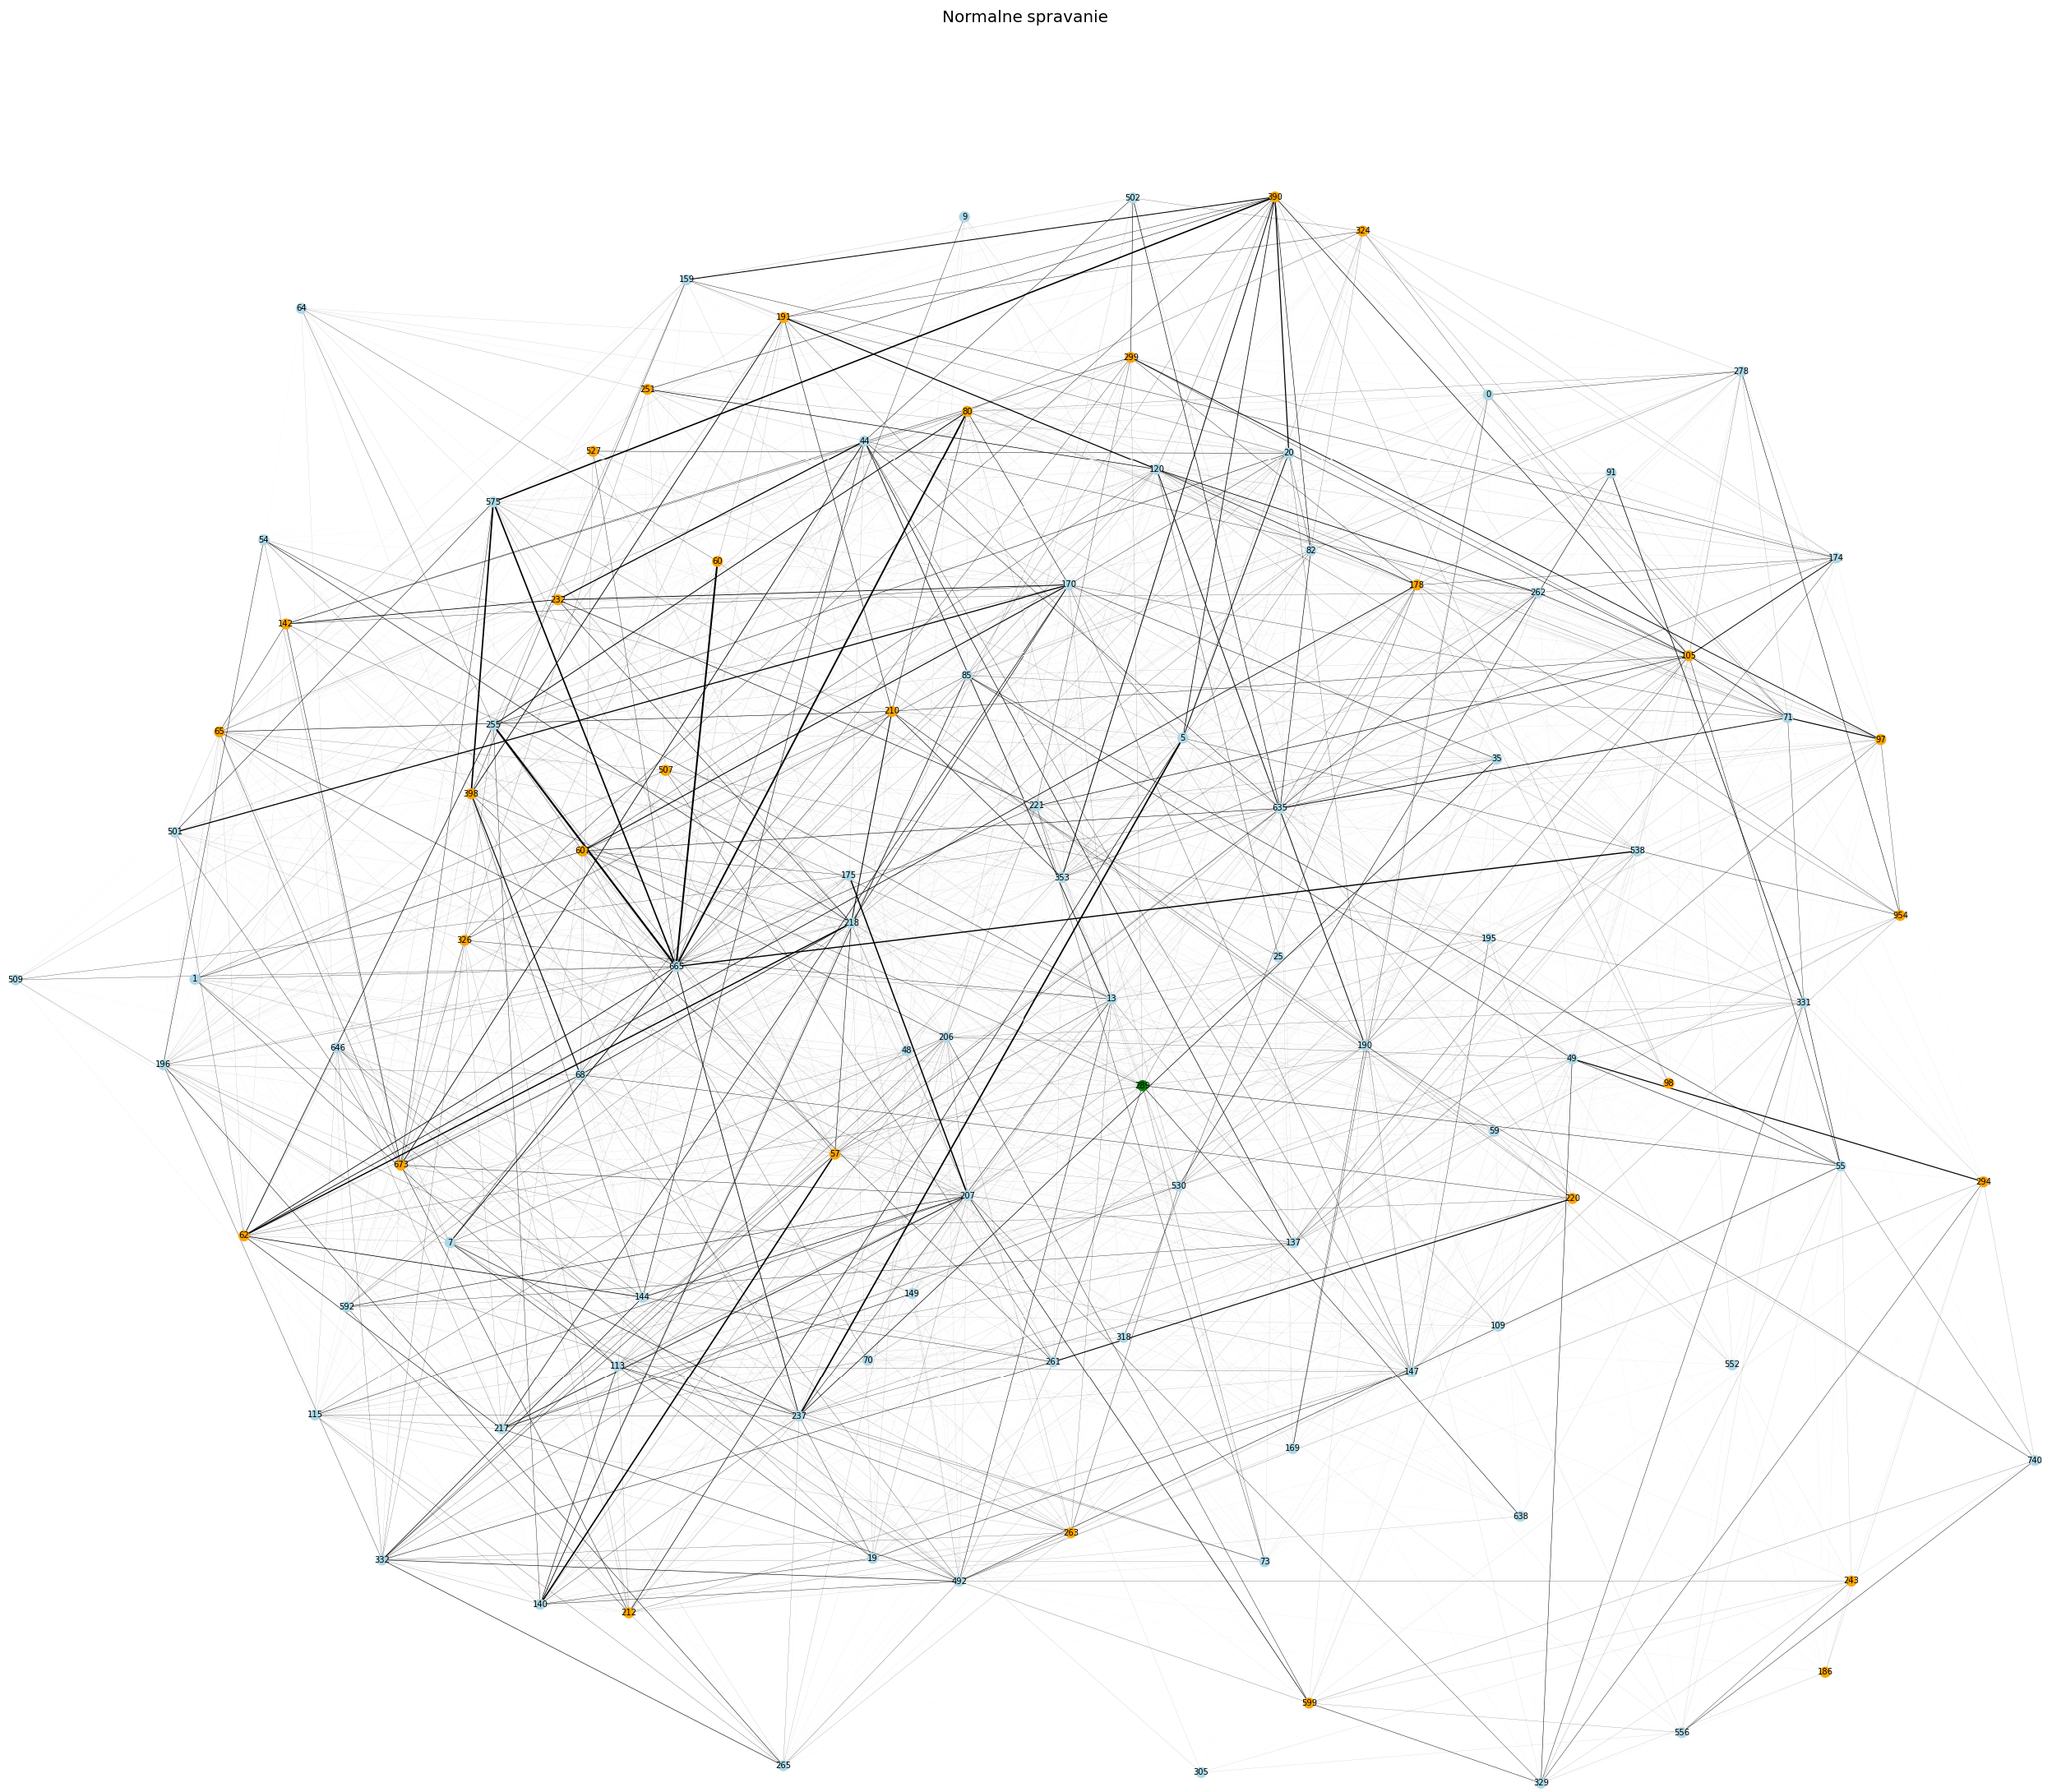
\includegraphics[width=0.7\textwidth]{norm_mravce}}
	
	V prípade náhodného správania mravcov vyzerala výsledná sieť následovne:
	
	\centerline{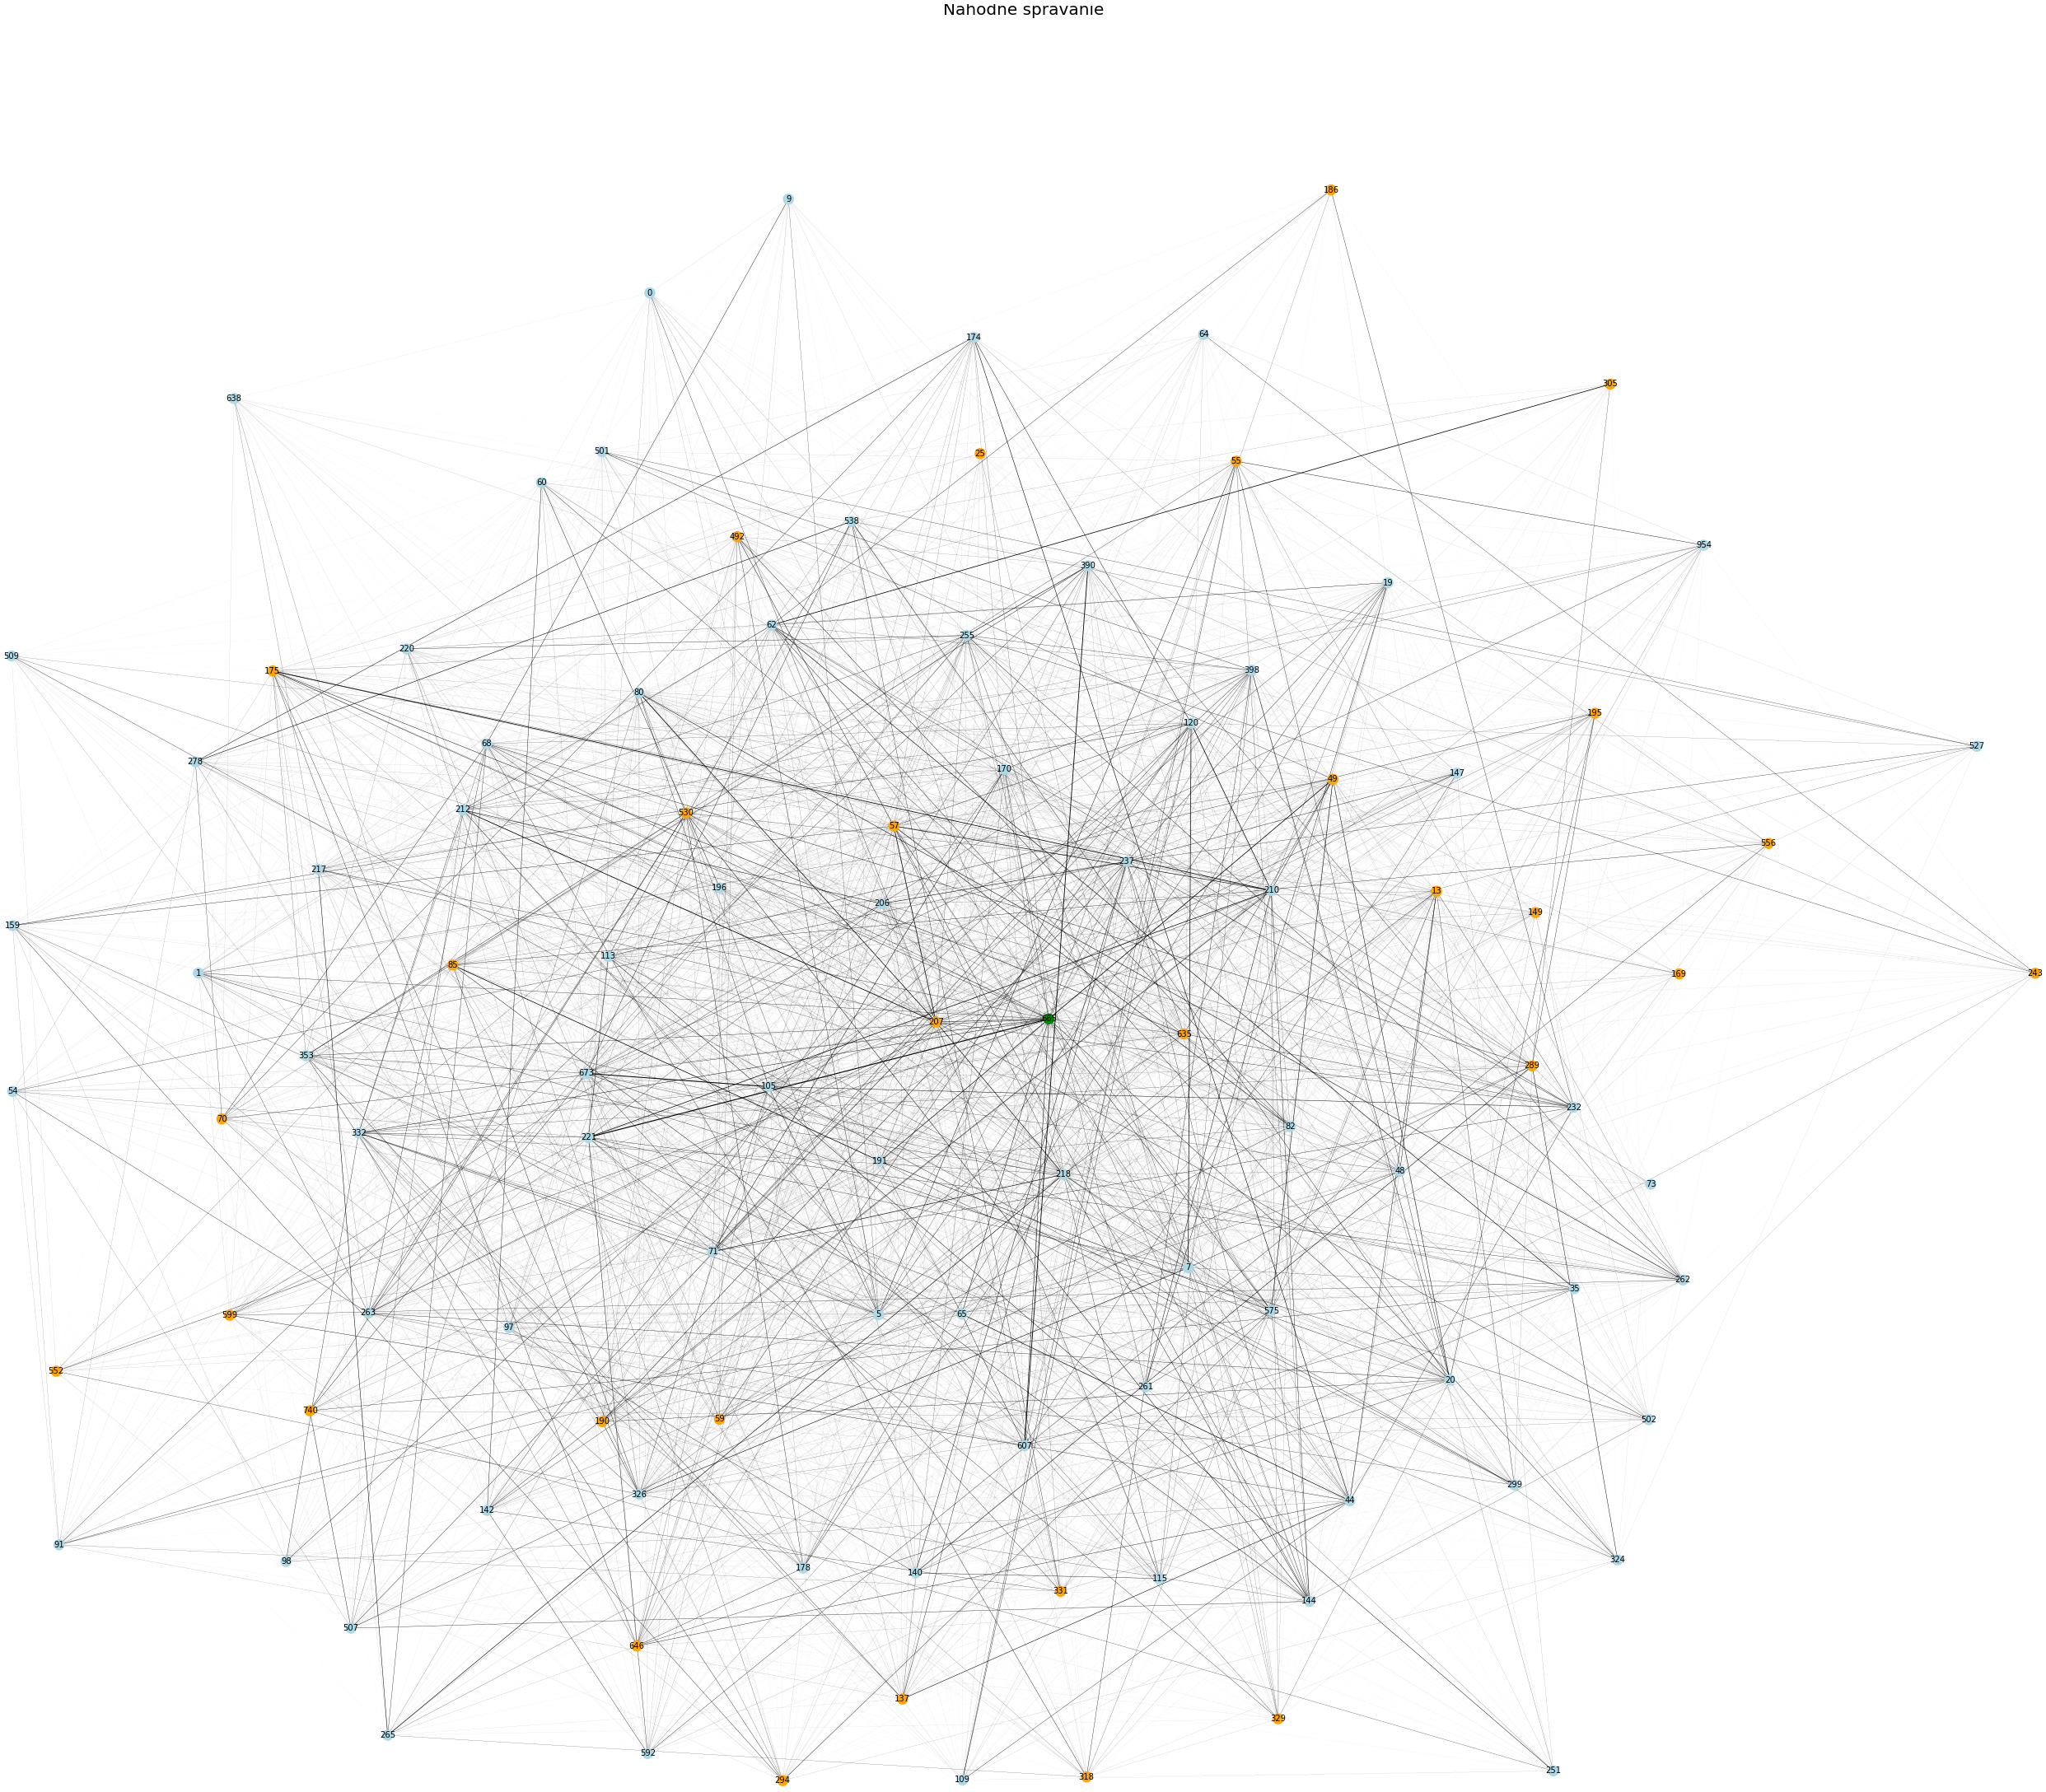
\includegraphics[width=0.7\textwidth]{rand_mravce}}
	
	V oboch grafoch sú mravce typu ''nurse'' označené svetlo modrou farbou, ''forager'' oranžovou a ''queen'' zelenou. Intenzita (v realite hrúbka) hrany udáva celkový čas kontaktu medzi dvojicou mravcov (čím tmavšia/hrubšia tým dlhší kontakt). (Obrázky vo vyššej kvalite v priloženej zložke ''kravec\_kod'') 
	
	\item 
	Na výpočet modularity sme využili funkciu z knižnice ''networkx'' konkrétne z triedy ''community'' metódu ''modularity'' (\href{https://networkx.org/documentation/stable/reference/algorithms/generated/networkx.algorithms.community.quality.modularity.html}{zdroj}). Táto funkcia používa na výpočet následovný vzorec: 
	\begin{gather*}
		Q = \sum_{c=1}^{n} \left[ \frac{L_c}{m} - \gamma \left( \frac{k_c}{2m} \right)^2 \right]
	\end{gather*}
	V tomto vzorci suma prechádza cez všetky komunity $c$ pričom $L_c$ je počet vnútro-komunitných prepojení, $k_c$ je suma stupňov vrcholov v komunite a $\gamma$ je ''resolution parameter'' ktorým je možné nastavovať či má funkcia preferovať veľké komunity ($\gamma<1$) alebo malé komunity ($\gamma>1$).

	Ide o redukovaná verzia vzorca:
	\begin{gather*}
		Q = \frac{1}{2m} \sum_{ij} \left( A_{ij} - \gamma \frac{k_{i}k_{j}}{2m} \right) \delta (c_i, c_j)
	\end{gather*}

	Výsledná modularita v sieti s reálnymi dátami je $0.0603$ a v náhodnej sieti je $-0.0023$. Takže modularita v reálnej sieti je kladná zatiaľ čo v náhodnej je záporná preto môžeme tvrdiť, že v reálnej sieti je výraznejšia klustrovanie vrcholov do komunít.
	
	\item 
	Na výpočet hustoty siete sme využili vzorec: 
	\begin{gather*}
		\rho = \frac{2m}{n(n-1)}
	\end{gather*}
	Výsledná hodnota reálnej siete vyšla $0.4007$ a náhodnej siete $0.6689$. Z toho vidíme, že náhodne vygenerovaná sieť je hustejšia.
	
	\item 
	Na výpočet hustoty siete sme využili vzorec: 
	\begin{gather*}
		\mu = \frac{m}{n}
	\end{gather*}
	Priemerný stupeň vrchola reálnej siete vyšiel $20.8381$ a náhodnej siete $34.7810$. Z toho vidíme, že náhodne vygenerovaná sieť má výrazne väčší stupeň vrcholu.
	
	\item 
	Vírus by sa mal lepšie šíriť v náhodne generovanej a to z dvoch dôvodov. Poprvé táto sieť má menšiu (zápornú) modularitu čo znamená, že sieť je tvorená jednou komunitou respektíve, že medzi komunitami je pomerne veľké množstvo interakcie vďaka čomu nie je šírenie vírusu nijak obmedzené, zatiaľ čo v reálnej sieti ktorá má väčšiu (kladnú) modularitu existujú komunity medzi v rámci ktorých šírenie vírusu nie je obmedzené ale je výrazne obmedzené šírenie medzi jednotlivými komunitami. Druhým dôvodom je vyššia hustota a priemerný stupeň vrchola náhodnej siete vďaka v priemere existuje viac jedincov (priamych kontaktov) ktorých môže chorý jedinec nakaziť.
	
	\item 
	Na spracovanie vstupných dát, vytvorenie sietí a výpočet štatistík siete sme použili programovací jazyk Python konkrétne knižnice ''pandas'' (na načítanie súboru) a ''networkx'' (na vytvorenie sietí a výpočet modularity), zároveň sme naprogramovali funkciu ''df\_matrix\_cleaner'' ktorej úlohou je vytvorenie matice susedností obsahujúcej súčty stretnutí. V priloženej zložke ''kravec\_kod'' sa nachádza súbor ''dataDU.xlsx'' obsahujúci vstupné dáta a súbor ''kravec\_siete.ipynb'' obsahujúci samotný kód na spracovanie grafov, ich vykreslenie a výpočet štatistík.

\end{enumerate}

\section{Úloha 2}

\begin{enumerate}[(a)]
	\item 
	Vieme, že gigantický komponent zahŕňa presne polovicu vrcholov čiže $S=0.5$, chceme zistiť priemerný stupeň vrcholu $c$ na čo môžeme použiť následujúcu rovnicu:
	\begin{gather*}
		S = 1 - e^{-cS} \\
		\text{Po dosadení $S$ dostaneme:} \\
		0.5 = 1 - e^{-0.5c} \\
		e^{-0.5c} = 0.5 \\
		-0.5c = ln(0.5) \\
		c = -2ln(0.5) \\
		c = 1.3863
	\end{gather*}
	Takže priemerný stupeň vrcholu v takejto Poiisonovskej sieti je $1.3863$.
	
	\item 
	V prípade určenia pravdepodobnosti vrchola stupňa 5 môžeme postupovať dvomi spôsobmi. Prvý spôsob je, že budeme uvažovať, že rozdelenie stupňa vrchola je binomické ($k\sim Bin(n-1,p)$) a v takom prípade pravdepodobnosť vrchola stupňa 5 je $P(k=5) = p^5(1-p)^{n-1-5}\binom{n-1}{5}$ avšak keďže nepoznáme $p$ ani $n$ a nie je možné ich z nami známych informácii vypočítať je táto pravdepodobnosť nevyčísliteľná. V prípade druhého postupu uvažujeme, že informácia ''s dostatočne veľkým $n$'' znamená, že môžeme uvažovať, že rozdelenie stupňa vrcholov je Poissonovske ($k \sim Poi(c)$) a v takomto prípade je pravdepodobnosť, že vrchol má stupeň 5 nasledovná $P(k=5) = \frac{c^5e^{-c}}{5!}$, keďže hodnotu $c$ už poznáme, môžeme túto hodnotu vyčísliť a dostaneme:
	\begin{gather*}
		P(k=5) = \frac{1.3863^5e^{-1.3863}}{5!} = 0.0107
	\end{gather*}
	Čiže pravdepodobnosť, že vrchol má stupeň 5 je približne 11\%.
	
	\item 
	Úprimne netuším ako správne postupovať v tejto úlohe. Logickou úvahou, ktorou som sa rozhodol túto úlohu riešiť je, že ak aspoň jeden zo susedov nášho vrcholu patrí do gigantického komponentu tak aj samotný vrchol musí do gigantického komponentu patriť. Podmienka ''aspoň jeden'' sa však komplikovane počíta a je jednoduchšie vypočítať inverznú úlohu ''ani jeden nepatrí'' a výsledná pravdepodobnosť je komplementom nami hľadanej pravdepodobnosti. Úlohu ani jeden nepatrí do gigantického komponentu môžeme počítať ako $u^k$ kde $u=1-S$ čiže pravdepodobnosť, že vrchol nepatrí do gigantického komponentu a $k$ je počet susedov čiže stupeň vrcholu. Keďže nás zaujíma komplement tejto úlohy dostaneme, že hľadaná pravdepodobnosť pre $k=5$ je $1-u^5 = 1-0.5^5 = 0.96875$ takže takmer 97\%.
	
	\item 
	Tento problém budeme riešiť následovne, poznáme pravdepodobnosť, že vrchol má stupeň 5 a pravdepodobnosť, že je v gigantickom komponente, vynásobením týchto pravdepodobností dostaneme pravdepodobnosť, že vrchol je stupňa 5 a je v gigantickom komponente. Na to aby sme zistili, aká je proporcia v gigantickom komponente máme 2 možnosti buď to jednoducho predelíme pravdepodobnosťou, že hociktorý vrchol patrí do gigantického komponentu čiže $S$ alebo súčtom pravdepodobností, že vrchol má stupeň $k$ a patrí do gigantického komponentu. Obe tieto spôsoby by mali dať rovnaký výsledok, čiže si môžeme skontrolovať, či náš vzorec na pravdepodobnosť, že vrchol stupňa $k$ patrí do gigantického komponentu. V ukážke nižšie použijeme verziu s predelením sumou.
	\begin{gather*}
		prop(k) = \frac{c^{k}e^{-c}(1-u^k)}{\sum_{i=0}^{n-1}c^{i}e^{-c}(1-u^i)} \\
		prop(5) = \frac{1.3863^{5}e^{-1.3863}(1-u^5)}{\sum_{i=0}^{n-1}1.3863^{i}e^{-1.3863}(1-u^i)} \\
		= \frac{0.0107*0.96875}{0.5} = \frac{0.0103}{0.5} = 0.0207
	\end{gather*}
	 
	Vidíme, že proporcia vrcholov stupňa 5 v gigantickom komponente je takmer 21\% zároveň si môžeme všimnúť, že menovateľ vyšiel presne 0.5 čo je naše $S$ čo hovorí, že náš vzorec na určenie pravdepodobnosti, že vrchol stupňa $k$ patrí do gigantického komponentu môže byť správny.
	
\end{enumerate}
 
\section{Úloha 3}

\begin{enumerate}[(a)]
	\item 
	V sieti kde každý vrchol má stupeň 1 nastáva situácia, že vrcholy tvoria dvojice keďže vo chvíli keď prepojíme 2 vrcholy hranou obe budú ''nasýtené'', čiže nebudú mať žiadnu voľnú polhranu. Z toho vyplýva, že všetky komponenty v grafe sú tvorený presne dvomi vrcholmi, čo je zanedbateľná veľkosť pre grafy ktoré nie su veľmi malá (2, 4 alebo 6 vrcholov) a zároveň graf obsahuje veľa rovnako veľkých komponentov preto môžeme tvrdiť, že takýto graf nemá gigantický komponent.
	
	\item 
	Pre grafy ktoré majú iba vrcholy jedného stupňa a to stupňa $k$ môžeme pravdepodobnostnú funkciu stupňa zapísať následovne:
	\begin{gather*}
		P(x) = \begin{cases} 1 & \text{ak } x = k \\
			0 & \text{ak } x \neq k      %
		\end{cases} \\
		p_x = \begin{cases} 1 & \text{ak } x = k \\
			0 & \text{ak } x \neq k      %
		\end{cases} \\
	\end{gather*} 
	
	Vieme, že vytvárajúca funkcia pre rozdelenie stupňa vrchola má následovný vzorec:
	\begin{gather*}
		g_0(u) = \sum_{i=0}^{\inf} p_iu^i
	\end{gather*} 

	Ale keďže mi vieme, že pre všetky $i\neq k$ je $p_i=0$ a pre $i=k$ je $p_k=1$ tak sa nám vzorec zjednoduchší na nasledovný:
	\begin{gather*}
		g_0(u) = u^k
	\end{gather*} 

	Vytvárajúcu funkciu pre rozdelenie stupňa susedného vrchola vieme vypočítať následovne:
	\begin{gather*}
		g_1(u) = \frac{g_0'(u)}{g_0'(1)}
	\end{gather*} 

	Najskôr si vypočítame deriváciu našej vytvárajúcej funkcie $g_0$:
	\begin{gather*}
		g_0(u) = u^k \\
		g_0(u) = ku^{k-1}
	\end{gather*}
	
	Keď to teraz dosadíme, do vzorca pre $g_1$ dostaneme:
	\begin{gather*}
		g_1(u) = \frac{g_0'(u)}{g_0'(1)} \\
		g_1(u) = \frac{ku^{k-1}}{k1^{k-1}} \\
		g_1(u) = \frac{ku^{k-1}}{k} \\
		g_1(u) = u^{k-1}
	\end{gather*} 

	Takže vytvárajúca funkcia pre rozdelenie stupňa vrchola je $g_0(u) = u^k$ a vytvárajúca funkcia pre rozdelenie stupňa susedného vrchola je $g_1(u) = u^{k-1}$.
	
	\item 
	Vieme, že veľkosť gigantického komponentu vieme v konfiguračnom modely vypočítať ako:
	\begin{gather*}
		S = 1- g_0(u)
	\end{gather*}  
	Z predchádzajúcej časti sme vypočítali, že $g_0(u) = u^k$, keďže v tomto prípade máme $k=3$ dostaneme, že veľkosť gigantického komponentu je: 
	\begin{gather*}
		S = 1- u^3
	\end{gather*}  
	teraz potrebujem vypočítať hodnotu $u$.
	
	Pre $u$ vieme, že platí rovnica:
	\begin{gather*}
		g_1(u) = u
	\end{gather*}
	V našom prípade kde $k=3$ vieme, že $g_1(u) = u^2$ po dosadení do predchádzajúcej rovnice dostaneme:
	\begin{gather*}
		u^2 = u \\
		u^2 - u = 0 \\
		u(u-1) = 0 \\
		u = \begin{cases} 0 \\ 1 \end{cases}
	\end{gather*}
	
	Ak tento výsledok dosadíme do našej rovnice pre S dostaneme následovné výsledky:
	\begin{gather*}
		S = 1 - u^3 \\
		S = \begin{cases} 1- 0^3 \\ 1- 1^3 \end{cases} \\
		S = \begin{cases} 1 \\ 0 \end{cases}
	\end{gather*}

	Z výsledkov vyplýva, že v grafe vytvoreným konfiguračným modelom kde všetky vrcholy majú stupeň 3 buď gigantický komponent neexistuje alebo pokrýva celý graf. Čomu úplne nerozumiem ale netuším kde som spravil chybu.
\end{enumerate}

\end{document}
